\section{Redes dinâmicas}
 \label{chap:redes-dinamicas}
 
 TODO --- Introduzir o processo de previsão de agrupamentos espaço temporais e sugira dois métodos básicos de previsão: Usar o livro Mitsa (2010) pagina 105 (clsutering of Time Series Data Steams, Time Series Clustering Using Global Characteristics. Mostre como cada um funciona com um exemplo. Vá nos artigos que apresentam estes métodos---

 
 Para redes dinâmicas, o foco é tipicamente em uma classe de redes e questões referentes às estrutura dessa classe de rede, como a estrutura evoluiu e como isso afeta sistemas dinâmicos na rede. As redes temporais normalmente são mais orientadas a dados - onde se investiga um conjunto de dados, suas estruturas e como, por exemplo, surtos epidêmicos se comportariam sobre ele. Em seguida, é questionado como essas observações se generalizam comparando os resultados para diferentes conjuntos de dados \cite{holme:colloquium}.

\subsection{Agrupamento de dados baseado em predição}
%Temporal Data Mining [Mitsa]
A tarefa de predição visa descobrir o valor futuro de um determinado atributo de dados. É uma área com variedade de aplicações em diversas áreas como meteorologia e detecção de doenças. Por exemplo, um médico gostaria de prever a reação de seus pacientes a um novo medicamento para diabetes, particularmente a duração dos episódios de hipoglicemia.
Na previsão de eventos, é desejável prever a ocorrência de um evento ou o número de ocorrências de um evento ou a duração de um evento, dada a existência de certas condições. Por exemplo, um médico acaba de colocar um de seus pacientes epilépticos em uma nova droga que é muito eficaz, mas após o início da terapia pode causar um grave ataque de enxaqueca. O médico gostaria de prever a duração desse ataque, considerando o conhecimento sobre a idade do paciente e o número e duração dos ataques epilépticos no último ano. Nos problemas de previsão de eventos que lidam com a previsão da duração de um evento pode ser modelada usando uma variável contínua e pode-se usar a regressão linear para sua previsão, onde a regressão linear é um dos métodos de regressão mais amplamente disponíveis \cite{Mitsa:2010}.
Na previsão de séries temporais, os dados são dados históricos obtidos em intervalos de tempo regulares. Informações sobre padrões passados podem ser usadas para prever padrões futuros. No exemplo da enxaqueca, os dados poderiam ser a duração dos ataques de enxaqueca de outros pacientes sobre a droga, juntamente com informações sobre suas idades, condições médicas preexistentes e gravidade da epilepsia.

TODO -- criar subsections 
\subsection{Método lahiri}
\label{lahiri}
\cite{lahiri2007} apresentam um algoritmo de predição em redes temporais, e que usa a ideia de que certas
interações sinalizam a ocorrência de outros em algum momento no futuro. Através de análises estatísticas
o algoritmo mede o atraso entre as interações, e com isso pode-se prever quando certas interações vão ocorrer
com base em observações passadas e atuais. Propõe-se a utilização de subgrafos frequentes e discute
como identificar subgrafos que são persistidos em redes temporais.
\cite{lahiri2008} em seguida propõe um novo problema de mineração de dados para redes dinâmicas:
detecção de todos os padrões de interação que ocorrem em intervalos de tempo regulares.
 
\subsection{O modelo Dynagraph}

O Dynagraph \cite{dynagraph} é um modelo computacional que permite, a partir de uma estrutura de dados simples, modelo de um Grafo ou Rede Dinâmica, representar com o mínimo custo de armazenamento a evolução de uma instância de observação e estudos. Ele acompanha a evolução dos conjuntos de um grafo: de nós e ligações (arcos e elos), como inserção/retirada ao longo do tempo, e mudança de suas características (posição, cor, forma, tamanho, e outras), por meio de um editor de características, apresentado na próxima subseção.

\subsubsection{Estrutura de dados}

(TODO - anexar imagem da estrutura JSON usada pelo Dynagraph)

\subsection{Editor de características}
O Editor de Características é uma extensão do software Dynagraph, que permite alterar os atributos visuais dos vértices e aresta de um grafo dinâmico.
Com ele pode-se criar novos tipos de dados e com isso diferenciar, por exemplo, focos de casos de dengue e tipos de dengue.
Essa extensão permite criar com os seguintes atributos: Rótulo, Opacidade, Escala, Espessura da Borda, Cor da Borda e Cor de Preenchimento. Outra opção é utilizar uma imagem.
 
A figura \ref{fig:edCaMenu} exibe a localização do Editor de Características na aplicação em um menu lateral com as seguinte opções: Vértice, Aresta e um painel, este exibe a data atual e número de vértices e arestas em análise.
\begin{figure}[!ht]
	\centering	
	\caption{\label{fig:edCaMenu} Editor de Características: menu lateral}
	\UECEfig{}{
		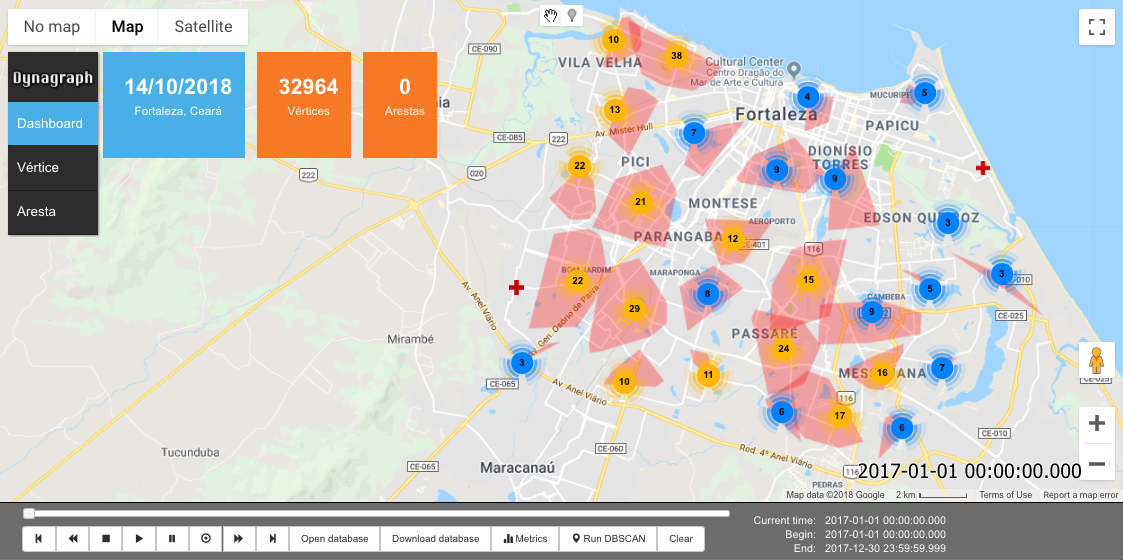
\includegraphics[width=15cm]{figuras/editorCaract/edCaractMenu.png}
	}{
		\Fonte{Elaborado pelo autor}
	}
\end{figure}
\FloatBarrier

Para criar um novo vértice deve-se selecionar o submenu relacionado a vértices como mostra a figura \ref{fig:edCaCriacao1}.
\begin{figure}[!ht]
	\centering	
	\Caption{\label{fig:edCaCriacao1} Editor de Características: criação de um vértice}	
	\UECEfig{}{
		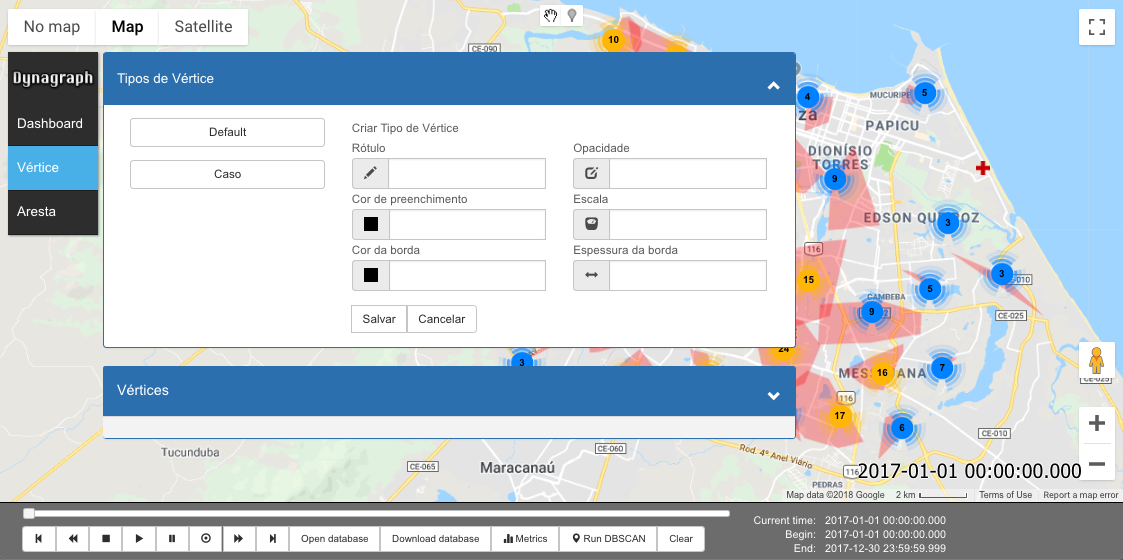
\includegraphics[width=15cm]{figuras/editorCaract/1edCaractCreateVertice.png}
	}{
		\Fonte{Elaborado pelo autor}
	}
\end{figure}
\FloatBarrier

A figura \ref{fig:edCaCriacao2} exibe os tipos de dados permitidos na criação ou edição de um vértice.
\begin{figure}[!ht]
	\centering	
	\Caption{\label{fig:edCaCriacao2} Editor de Características: criação de um vértice - tipos de dados}	
	\UECEfig{}{
		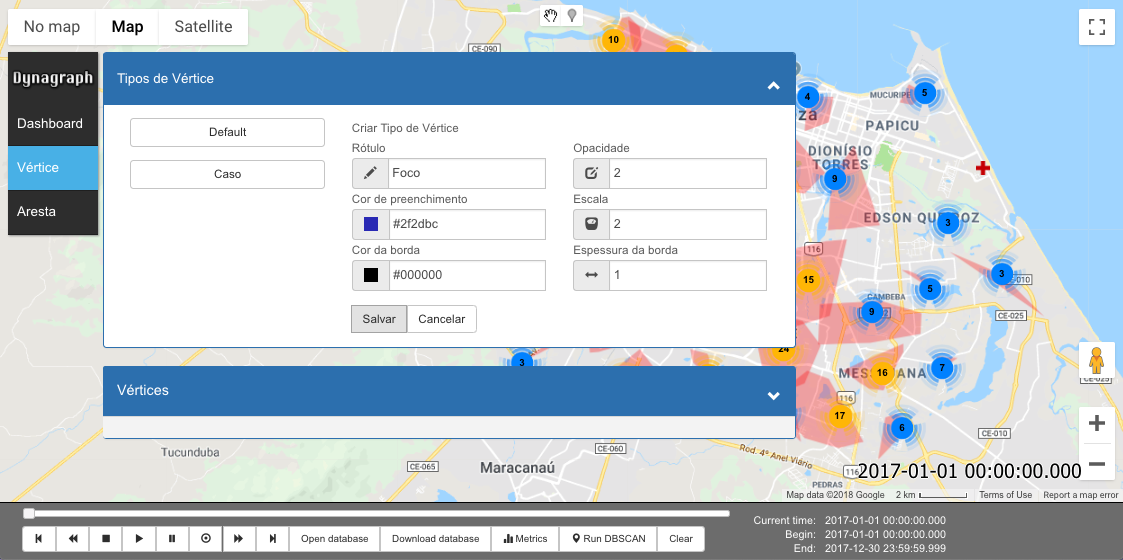
\includegraphics[width=15cm]{figuras/editorCaract/2edCaractCreateVertice.png}
	}{
		\Fonte{Elaborado pelo autor}
	}
\end{figure}
\FloatBarrier

Após criar um novo tipo de vértice pode-se usá-lo editando um dado ponto no mapa, como mostram as figuras \ref{fig:edCaChangeV1} e \ref{fig:edCaChangeV2}.
A figura \ref{fig:edCaShowV} exibe o resultado esperado.
\begin{figure}[!ht]
	\centering	
	\Caption{\label{fig:edCaChangeV1} Editor de Características: edição de um vértice - parte 1}	
	\UECEfig{}{
		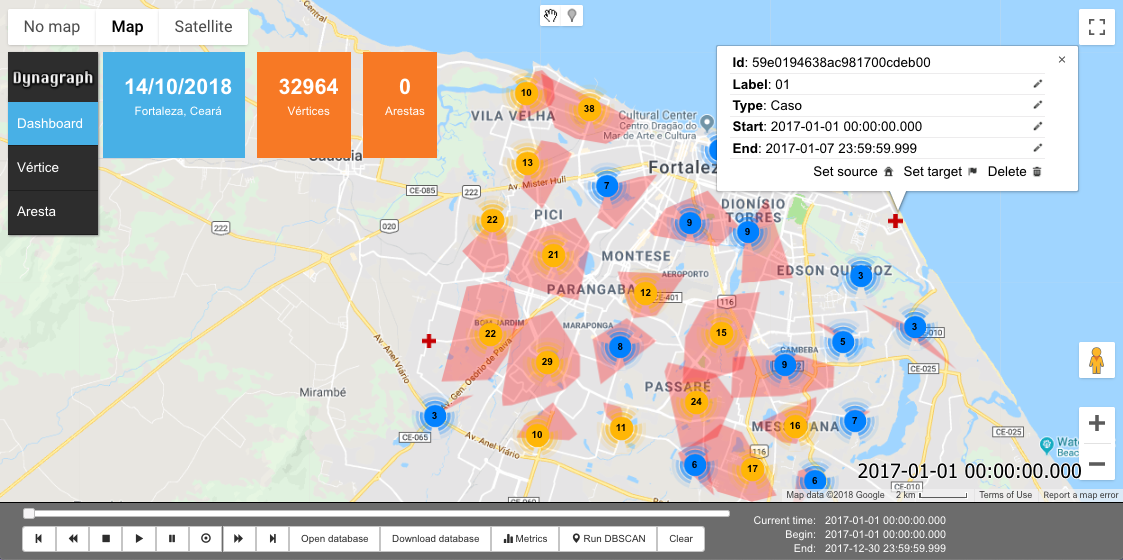
\includegraphics[width=15cm]{figuras/editorCaract/3edCaractChangeVertice.png}
	}{
		\Fonte{Elaborado pelo autor}
	}
\end{figure}
\FloatBarrier

\begin{figure}[!ht]
	\centering	
	\Caption{\label{fig:edCaChangeV2} Editor de Características: edição de um vértice - parte 2}	
	\UECEfig{}{
		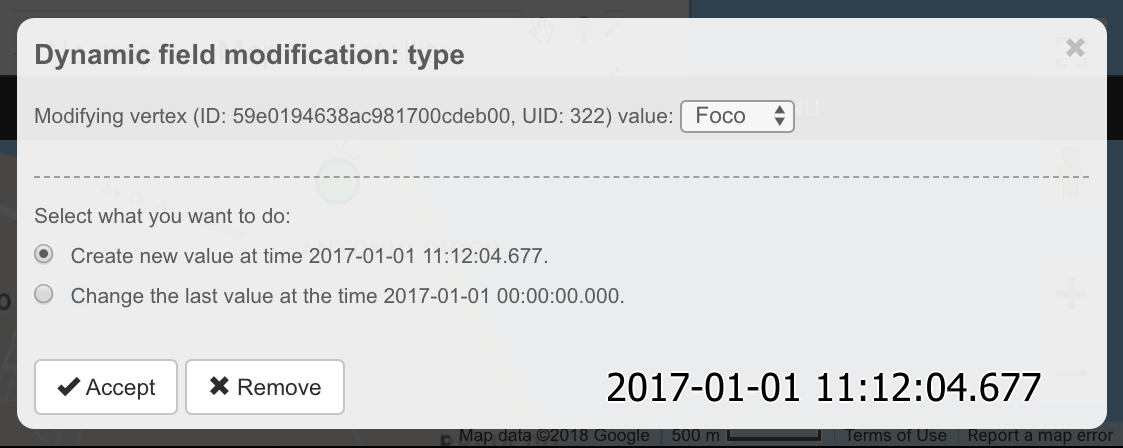
\includegraphics[width=15cm]{figuras/editorCaract/4edCaractChangeVertice.png}
	}{
		\Fonte{Elaborado pelo autor}
	}
\end{figure}
\FloatBarrier

\begin{figure}[!ht]
	\centering	
	\Caption{\label{fig:edCaShowV} Editor de Características: edição de um vértice - parte 3}	
	\UECEfig{}{
		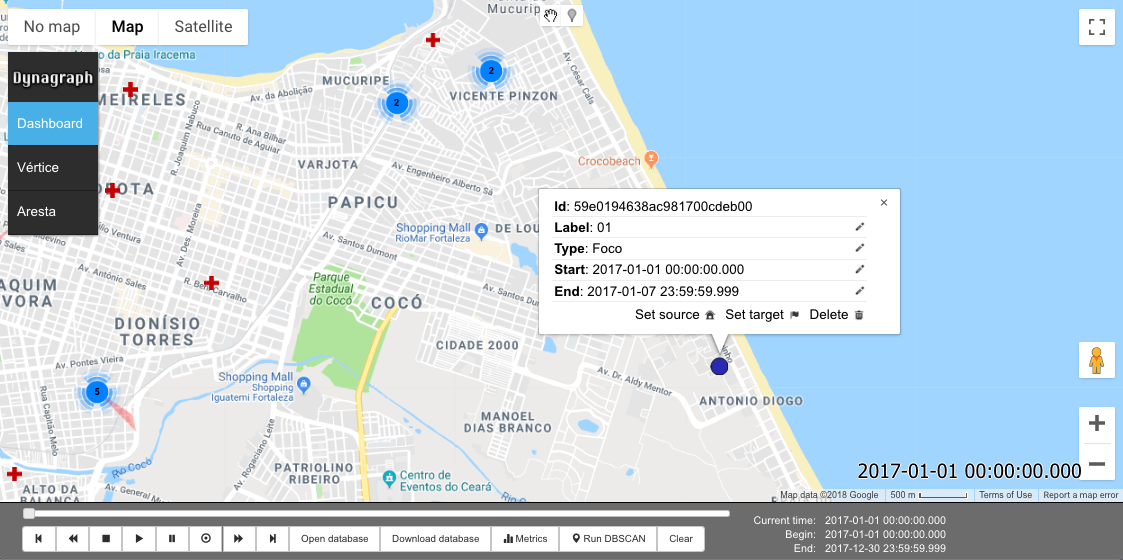
\includegraphics[width=15cm]{figuras/editorCaract/5edCaractShowVertice.png}
	}{
		\Fonte{Elaborado pelo autor}
	}
\end{figure}
\FloatBarrier

Para editar um tipo de vértice basta selecioná-lo a partir da lista de tipos de vértices e então aplicar as mudanças, como mostra a figura \ref{fig:edCaEditV1} e o resultado na figura \ref{fig:edCaEditV2}.
\begin{figure}[!ht]
	\centering	
	\Caption{\label{fig:edCaEditV1} Editor de Características: edição de um tipo de vértice - parte 1}	
	\UECEfig{}{
		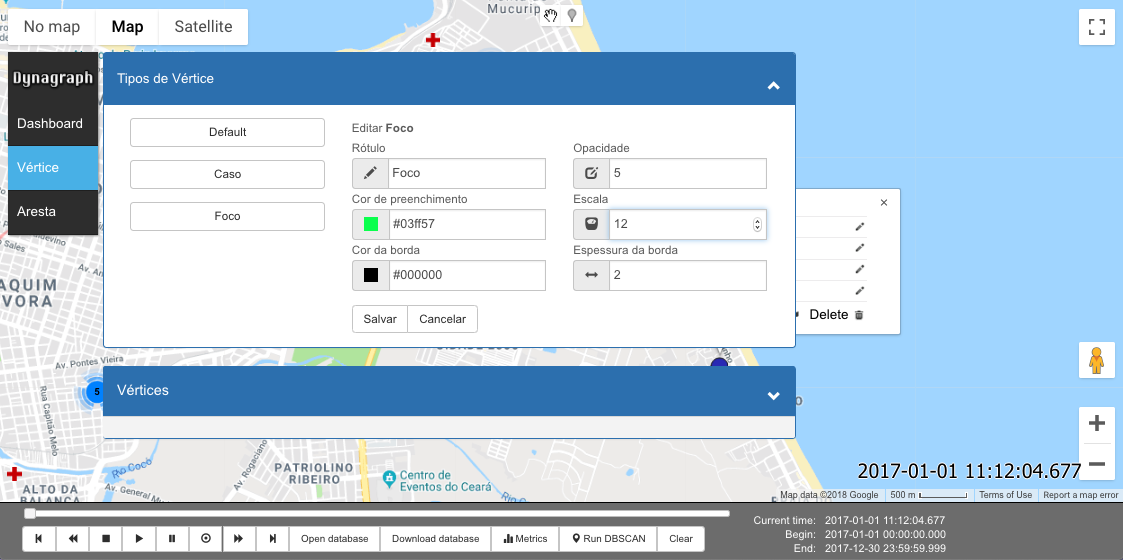
\includegraphics[width=15cm]{figuras/editorCaract/6edCaractEditVertice.png}
	}{
		\Fonte{Elaborado pelo autor}
	}
\end{figure}
\FloatBarrier
\begin{figure}[!ht]
	\centering	
	\Caption{\label{fig:edCaEditV2} Editor de Características: edição de um tipo de vértice - parte 2}	
	\UECEfig{}{
		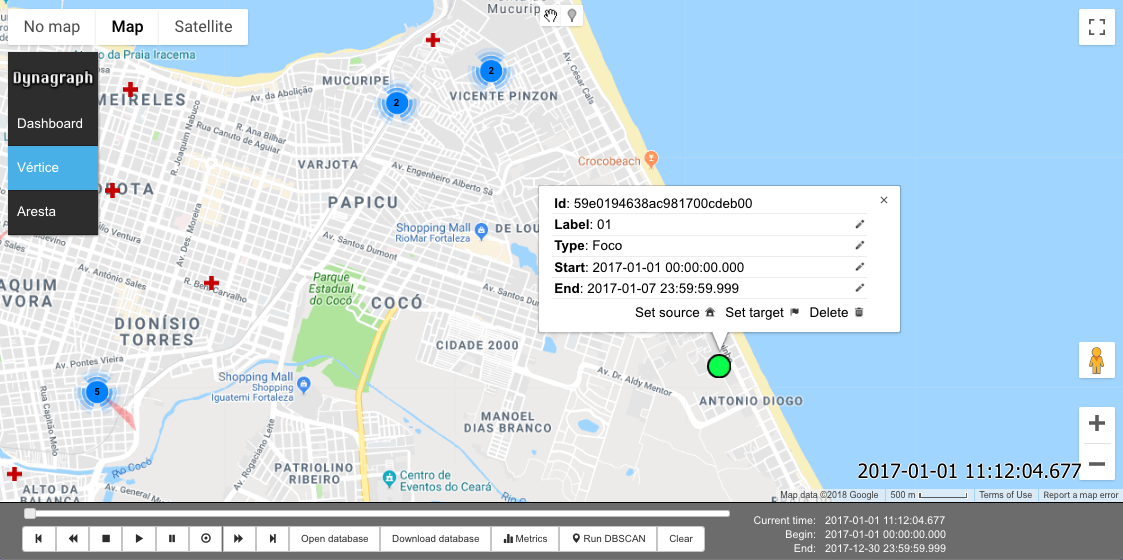
\includegraphics[width=15cm]{figuras/editorCaract/7edCaractEditedVertice.png}
	}{
		\Fonte{Elaborado pelo autor}
	}
\end{figure}
\FloatBarrier

Outra opção de edição de um vértice é dado na figura \ref{fig:edCaractEditVerticeOption2}. Nesta opção pode-se usar uma imagem pronta.
\begin{figure}[!ht]
	\centering	
	\Caption{\label{fig:edCaractEditVerticeOption2} Editor de Características: Tipo de vértice}	
	\UECEfig{}{
		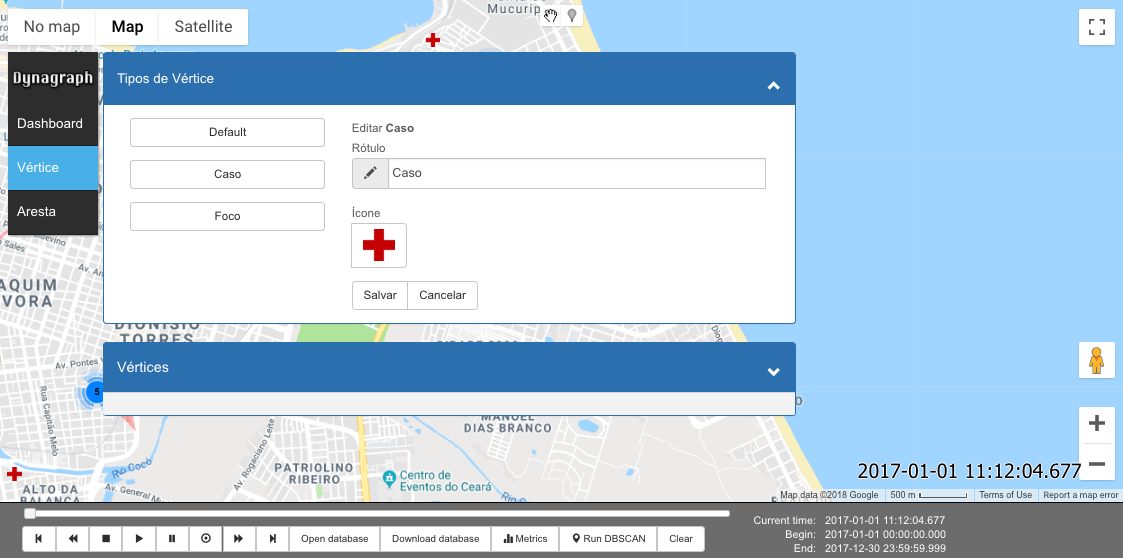
\includegraphics[width=15cm]{figuras/editorCaract/edCaractEditVerticeOption2.png}
	}{
		\Fonte{Elaborado pelo autor}
	}
\end{figure}
\FloatBarrier

O Editor de Características permite também a criação e edição de arestas (figura \ref{fig:edCaractAresta}), mas essa funcionalidade não foi necessária nesta pesquisa.
\begin{figure}[!ht]
	\centering	
	\Caption{\label{fig:edCaractAresta} Editor de Características: Aresta}	
	\UECEfig{}{
		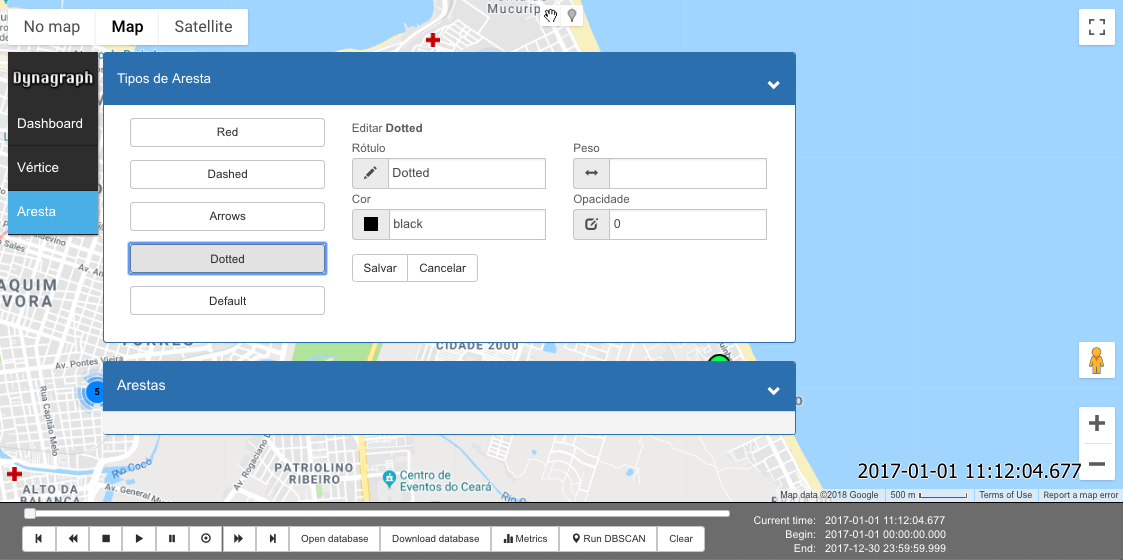
\includegraphics[width=15cm]{figuras/editorCaract/edCaractAresta.png}
	}{
		\Fonte{Elaborado pelo autor}
	}
\end{figure}
\FloatBarrier

\subsection{Visualização dos grupos formados}
Foram usados dois algoritmos para permitir a visualização dos grupos formados em um dado tempo.
O primeiro é uma biblioteca da API do Google chamada MarkerClusterer \cite{markerCluster} que cria e gerencia grupos de acordo com o nível de zoom para grandes quantidades de pontos.
Essa biblioteca é combinada com a API Javascript do Google Maps para agrupar os pontos por proximidade em grupos e simplificar a exibição dos pontos no mapa.
De acordo com o nível de zoom os grupos são formados com cores e tamanhos diferentes, como mostra as figuras \ref{fig:apiGoogleMaps1} e \ref{fig:apiGoogleMaps2}.
\begin{figure}[!ht]
	\centering	
	\Caption{\label{fig:apiGoogleMaps1} Grupos - API Google Maps parte 1}	
	\UECEfig{}{
		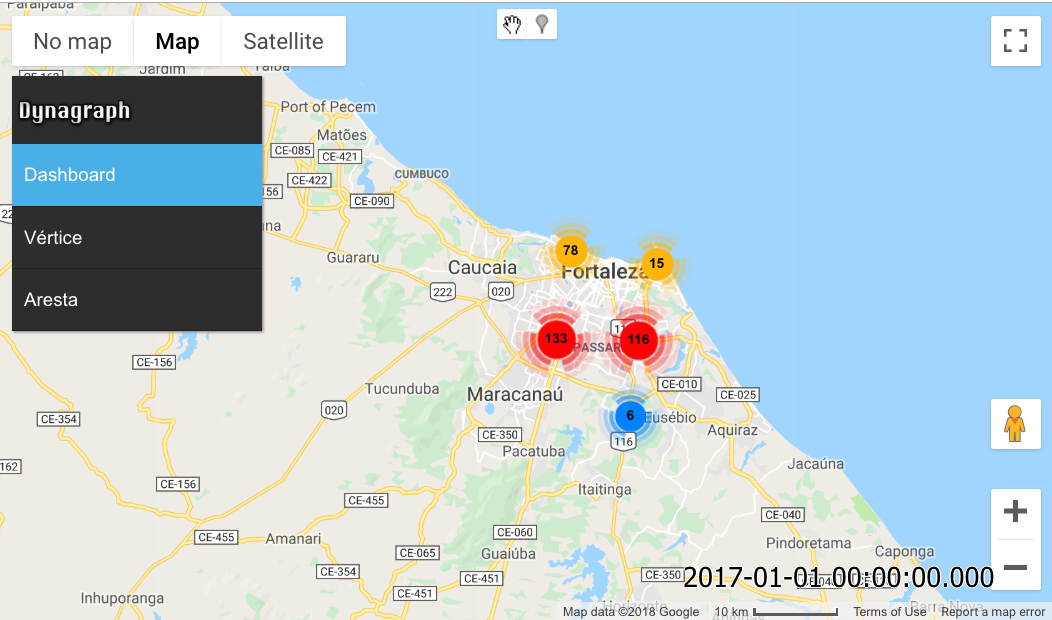
\includegraphics[width=13cm]{figuras/ClusterAPIGoogle1.png}
	}{
		\Fonte{Elaborado pelo autor}
	}
\end{figure}
\FloatBarrier

\begin{figure}[!ht]
	\centering	
	\Caption{\label{fig:apiGoogleMaps2} Grupos - API Google Maps parte 2}	
	\UECEfig{}{
		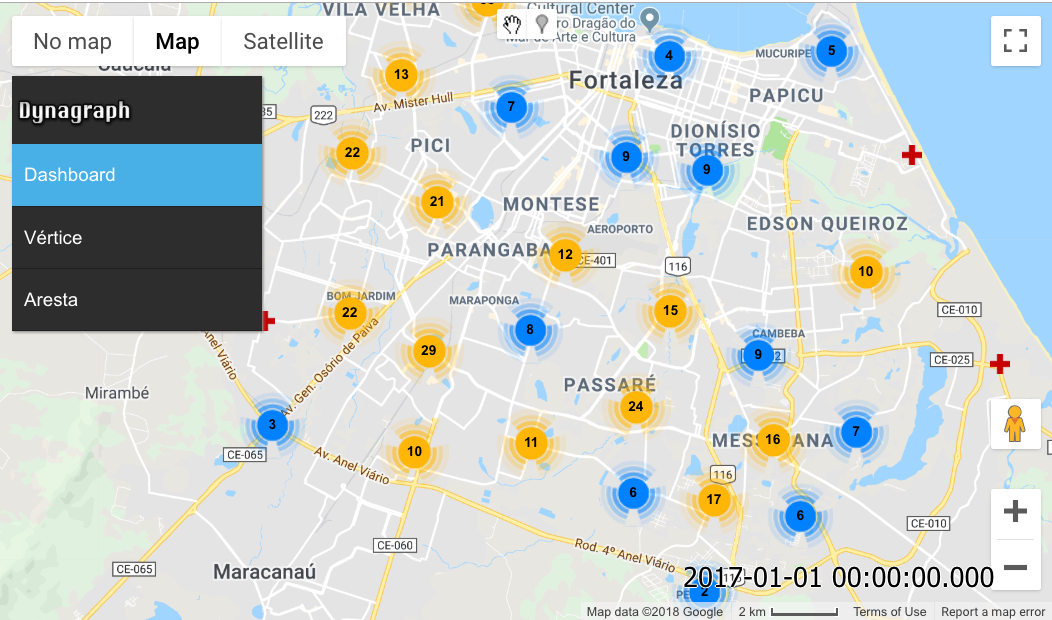
\includegraphics[width=13cm]{figuras/ClusterAPIGoogle2.png}
	}{
		\Fonte{Elaborado pelo autor}
	}
\end{figure}
\FloatBarrier

O segundo algoritmo é conhecido como Convex Hull \cite{ConvexHull}. Também conhecido como fecho convexo onde, dado um conjunto de pontos em um espaço,
o problema consiste em encontrar o menor número de pontos que gerem um polígono convexo no qual abranja todos os outros pontos.
As figuras \ref{fig:algConvexHull1} e \ref{fig:algConvexHull2} são exemplos do convex hull, onde cada polígono representa o grupo de casos de dengue naquela região delimitada. Dos vários pontos, somente os pontos mais externos e que formam o menor polígono que englobam todos os outros pontos.
%
\begin{figure}[!ht]
	\centering	
	\Caption{\label{fig:algConvexHull1} Exemplo 1 de Convex Hull}	
	\UECEfig{}{
		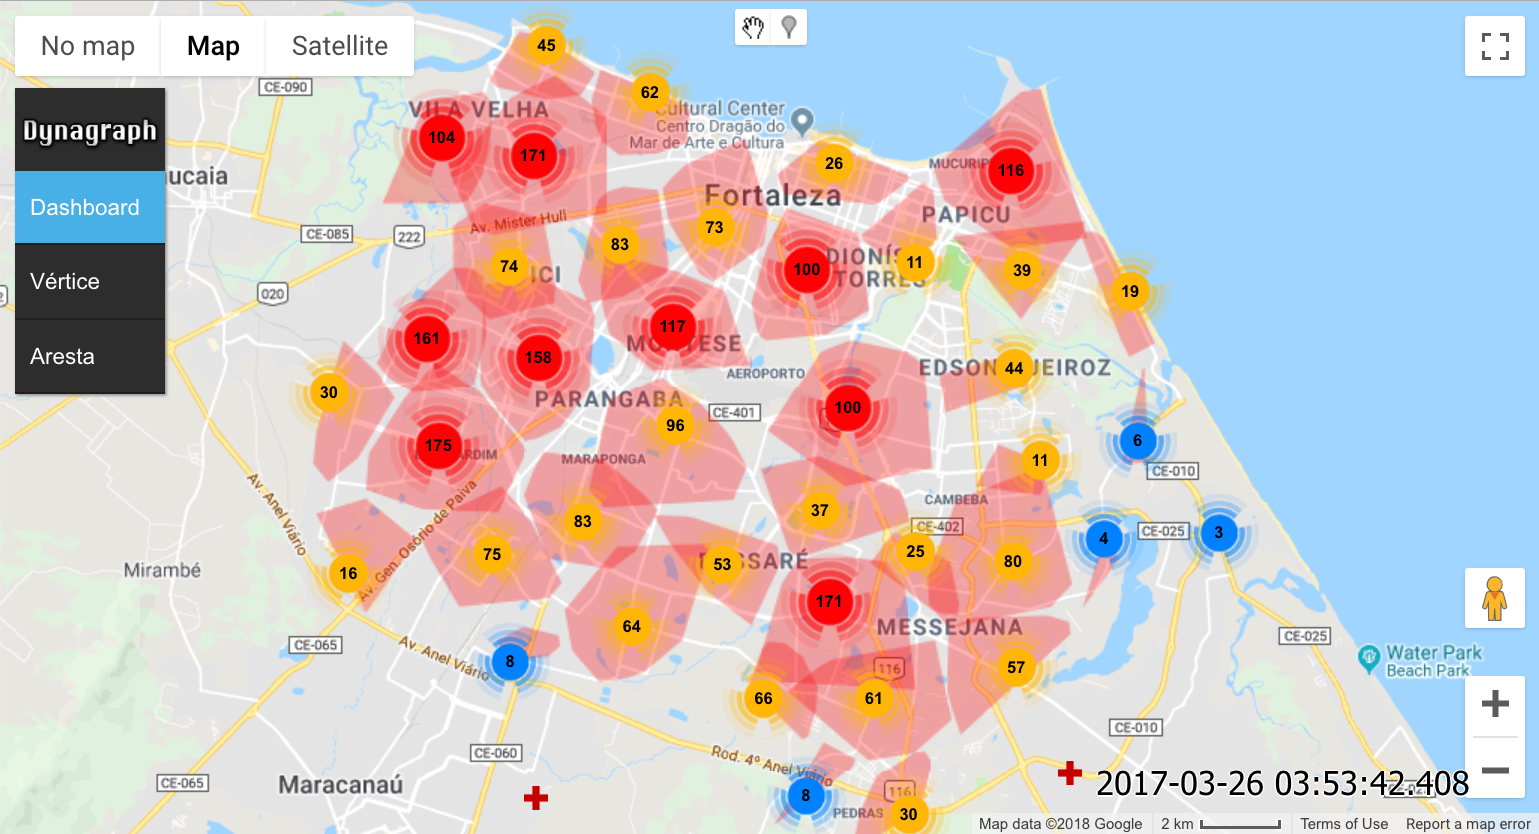
\includegraphics[width=14cm]{figuras/algConvexHull1.png}
	}{
		\Fonte{Elaborado pelo autor}
	}
\end{figure}
\FloatBarrier
\begin{figure}[!ht]
	\centering	
	\Caption{\label{fig:algConvexHull2} Exemplo 2 de Convex Hull}	
	\UECEfig{}{
		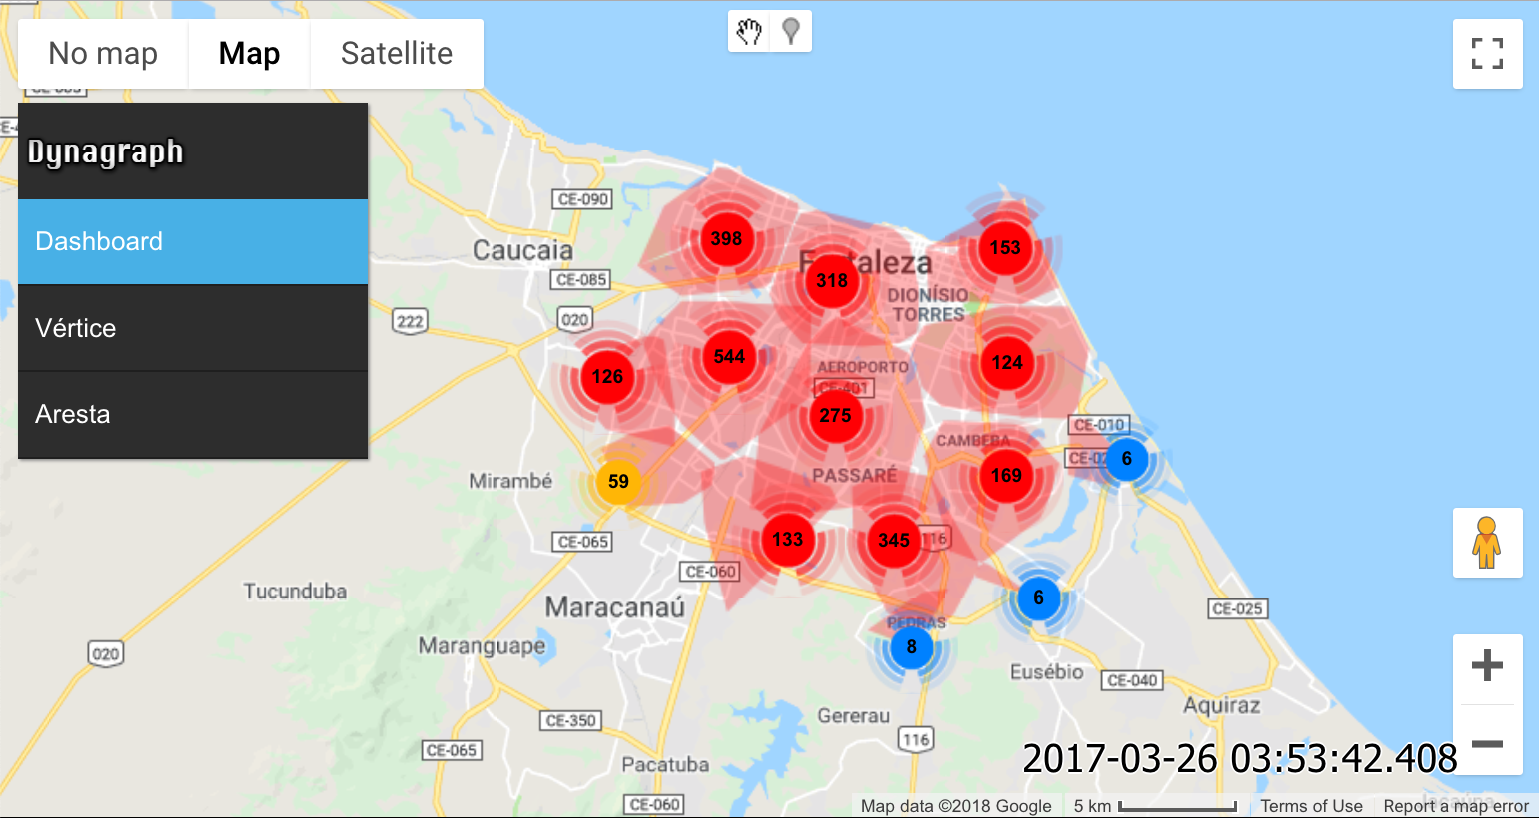
\includegraphics[width=14cm]{figuras/algConvexHull2.png}
	}{
		\Fonte{Elaborado pelo autor}
	}
\end{figure}
\FloatBarrier
